\documentclass[aspectratio=169,10pt]{beamer}

\usetheme{Madrid}
\usecolortheme{seahorse}
\usefonttheme{professionalfonts}

\usepackage{amsmath,amssymb,amsthm}
\usepackage{mathtools}
\usepackage{listings}
\usepackage{xcolor}
\usepackage{booktabs}
\usepackage{graphicx}
\usepackage{algorithm}
\usepackage{algpseudocode}
\usepackage{multirow}
\usepackage{enumerate}
\usepackage{tikz}
\usetikzlibrary{arrows.meta, positioning, shapes.geometric}

\graphicspath{{figures/}}

%% Python style
\lstdefinestyle{python}{
  language=Python,
  basicstyle=\ttfamily\scriptsize,
  keywordstyle=\color{blue!80!black}\bfseries,
  stringstyle=\color{orange!80!black},
  commentstyle=\color{green!50!black}\itshape,
  numberstyle=\tiny\color{gray},
  numbers=left, stepnumber=1,
  frame=single, breaklines=true,
  showstringspaces=false, tabsize=4,
  backgroundcolor=\color{gray!7},
}

\title[Bayesian ML in QF -- Ch.4]{Bayesian Machine Learning in Quantitative Finance}
\subtitle{Chapter 4: Volatility Surfaces with Sparse Gaussian Processes}
\author{Based on Mongwe, Mbuvha \& Marwala}
\date{}

\setbeamertemplate{navigation symbols}{}
\setbeamertemplate{footline}[frame number]

\begin{document}

% ------------------------------------------------------------------------------ title
\begin{frame}
  \titlepage
\end{frame}

% ------------------------------------------------------------------------------ TOC
\begin{frame}{Chapter 4 Outline}
  \tableofcontents
\end{frame}

% ==============================================================================
\section{4.1 Introduction}
% ==============================================================================

\begin{frame}[allowframebreaks]{4.1 Why Volatility Surfaces? Why Bayesian ML?}

Chapters so far in this series have used Markov chain Monte Carlo (MCMC) and
related Bayesian tools to fit models to data. This chapter turns to a
concrete, high-stakes application in finance: \textbf{fitting stochastic
volatility models to the market's option prices}, a task called
\emph{calibration}.

\begin{block}{The Practical Problem}
Every day, an equity index (say the FTSE/JSE All Share Index or the
EuroStoxx 50) has hundreds of options trading at different strikes and
maturities. A trading desk needs a \emph{single, consistent model} of how
the underlying's volatility behaves, so that it can price, hedge, and risk
manage options that are \emph{not} directly quoted in the market. Fitting
such a model to today's option prices is called \textbf{model calibration}.
\end{block}

\framebreak

\textbf{Two obstacles making calibration hard:}
\begin{itemize}
  \item \textbf{Cost:} realistic stochastic volatility models (Section 4.2)
        often have no simple closed-form option pricing formula, so
        pricing a single option can require an expensive Monte Carlo
        simulation. Calibrating means pricing \emph{many} options,
        \emph{many} times, while an optimizer searches over parameters --
        this can be prohibitively slow if done na\"ively.
  \item \textbf{Ill-posedness:} calibration is an \emph{inverse problem} --
        many different parameter combinations can produce nearly the same
        option prices, so the ``best fit'' is not unique and small data
        errors can cause large parameter swings. This calls for
        \emph{regularization}.
\end{itemize}

\begin{alertblock}{The Machine Learning Fix}
Recent literature (Horv\'ath et al., 2021) trains a neural network
\emph{offline} to learn the mapping from model parameters to option prices
(or implied volatilities). Once trained, this network is a nearly-instant
\textbf{surrogate} for the expensive pricing step, so calibration to real
market data becomes a fast optimization against the surrogate instead of
against a slow Monte Carlo pricer.
\end{alertblock}

\framebreak

\textbf{Why go further and use Gaussian processes (GPs) instead of (or
alongside) neural networks?}
\begin{itemize}
  \item Neural networks are black boxes: hard to interpret, and one must
        hand-pick an architecture (number of layers, neurons, activation)
        with no canonical recipe.
  \item Bayesian methods, including GPs, naturally regularize through a
        \emph{prior distribution} -- helpful for an ill-posed problem.
  \item GPs additionally report \textbf{uncertainty} on every prediction
        (and hence on every calibrated parameter), which a plain neural
        network does not.
  \item Drawback: GPs are much more computationally expensive to train
        than neural networks (cubic in the number of training points) --
        motivating the \emph{sparse} GP machinery covered later in this
        chapter.
\end{itemize}

This chapter's contribution: a first-in-the-literature Bayesian
(Gaussian process) framework for learning volatility surfaces, applied to
\emph{both} a developing market (South Africa's FTSE/JSE ALSI) and a
developed market (EuroStoxx 50), and compared head-to-head against deep
neural networks.

\end{frame}

\begin{frame}[allowframebreaks]{4.1 What Is an Implied Volatility Surface?}

\begin{block}{Plain-Language Definition}
Take every quoted price of a stock-index option and plug it \emph{backwards}
into the Black--Scholes formula, solving for whatever constant volatility
number $\sigma$ would have produced that exact market price. This number is
the \textbf{implied volatility} for that option's strike $K$ and maturity
$T$. Plotting $\sigma_{\mathrm{imp}}(K,T)$ over the grid of all traded
strikes and maturities gives the \textbf{implied volatility surface}.
\end{block}

\textbf{The punchline:} if Black--Scholes were literally true, this surface
would be perfectly flat -- one $\sigma$ for every strike and maturity.
Real markets do not behave this way. Plotted implied volatilities dip and
curve, forming a \textbf{smile} (U-shape across strike) or a
\textbf{skew} (a downward slope, common in equity index options because
investors pay up for downside/crash protection).

\begin{columns}
  \column{0.55\textwidth}
    This is direct evidence that the market does \emph{not} believe
    volatility is constant -- it believes volatility itself is random and
    can jump, which is exactly what a \textbf{stochastic volatility model}
    (Section 4.2) is built to capture.
  \column{0.42\textwidth}
    \centering
    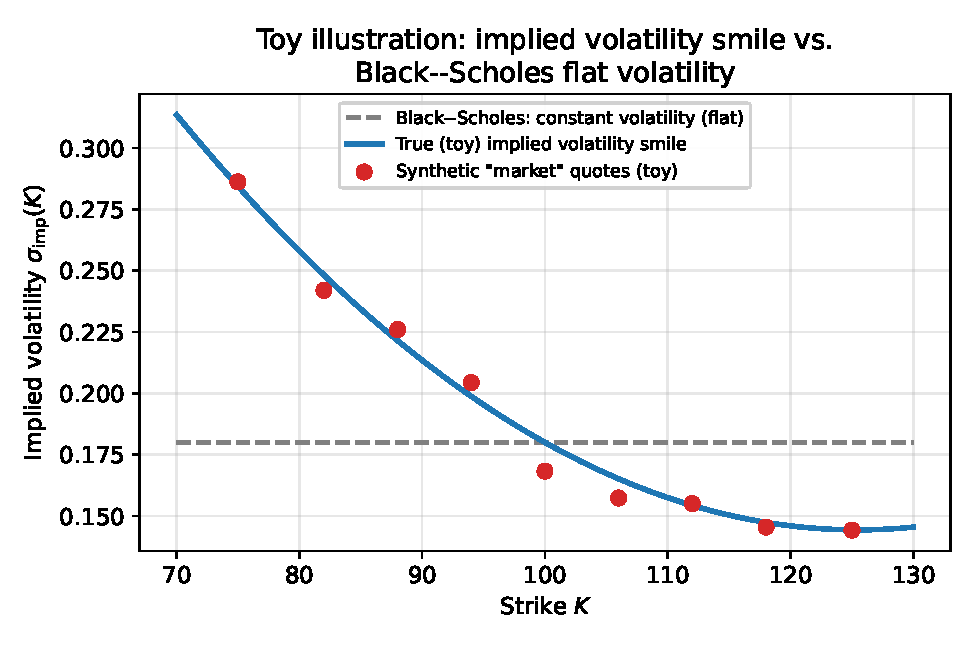
\includegraphics[width=\textwidth]{toy_smile}
\end{columns}

\framebreak

\textbf{Reading the toy figure above:}
\begin{itemize}
  \item The dashed grey line is what Black--Scholes assumes: one flat
        volatility number, regardless of strike.
  \item The blue curve is a toy (illustrative, not real-market) implied
        volatility smile: higher for low strikes (deep out-of-the-money
        puts / crash protection), a minimum somewhere near the
        at-the-money strike, and a mild upturn for high strikes.
  \item The red dots are synthetic ``market quotes'' -- noisy observations
        of the underlying smile, exactly like real bid/ask-derived
        implied volatilities.
\end{itemize}

The goal of \emph{calibration} is: given quotes like the red dots (at a
handful of strikes and maturities), find the stochastic volatility model
parameters that best reproduce this whole curved shape -- not just a
single flat number.

\end{frame}

\begin{frame}{4.1 Chapter Roadmap}
  \begin{block}{What This Chapter Covers}
    \begin{enumerate}
      \item \textbf{Sec.\ 4.2} -- Two stochastic volatility models: Heston
            and Rough Bergomi.
      \item \textbf{Sec.\ 4.3} -- The calibration framework, and the two
            machine learning surrogates: deep neural networks and
            (sparse) Gaussian processes.
      \item \textbf{Sec.\ 4.4} -- Numerical experiment setup: real option
            data from two equity markets, and the training/calibration
            protocol.
      \item \textbf{Sec.\ 4.5} -- Results: speed, parameter stability,
            fit quality, and the value of GP uncertainty bands.
      \item \textbf{Sec.\ 4.6} -- Conclusion and open questions.
    \end{enumerate}
  \end{block}
  \begin{alertblock}{First-in-Literature Claims (per the authors)}
    \begin{itemize}
      \item First Bayesian (GP-based) framework for learning volatility
            surfaces across both developed \emph{and} developing equity
            markets.
      \item First use of \textbf{sparse} Gaussian processes to calibrate
            stochastic volatility models to real financial market data.
    \end{itemize}
  \end{alertblock}
\end{frame}

% ==============================================================================
\section{4.2 Stochastic Volatility Models}
% ==============================================================================

\begin{frame}[allowframebreaks]{4.2 What Is a Stochastic Volatility Model?}

\begin{block}{Plain-Language Definition}
In the Black--Scholes world, volatility $\sigma$ is a fixed number that
never changes. A \textbf{stochastic volatility model} instead treats
volatility (or variance) as its \emph{own random process}, evolving through
time and driven by its own source of randomness -- typically correlated
with the randomness driving the asset price itself. This lets the model
generate exactly the kind of smiles/skews shown in the previous section.
\end{block}

Throughout Section 4.2, we work on a filtered probability space
$(\Omega, \mathcal{F}, (\mathcal{F}_t)_{t\in\mathbb{R}}, \mathbb{Q})$ which
supports \textbf{correlated Brownian motions} -- meaning we have two (or
more) Brownian motion processes $W_t^S$ (driving the asset price) and
$W_t^v$ (driving the variance), whose increments are correlated with each
other through a parameter $\rho$.

\framebreak

\textbf{Why bother with two separate models (Heston \emph{and} Rough
Bergomi) in this chapter?} They sit at two different points on a
trade-off:

\begin{itemize}
  \item \textbf{Heston} (Sec.\ 4.2.1): a classical, Markovian model.
        Analytically tractable (closed-form pricing exists via its
        characteristic function), well understood, but needs 4--5
        parameters and does not always fit the very short-maturity skew
        well.
  \item \textbf{Rough Bergomi} (Sec.\ 4.2.2): a modern ``rough
        volatility'' model. Uses a \emph{fractional} Brownian motion, is
        \emph{not} Markovian, has no simple closed-form price (Monte
        Carlo is typically required), but fits a much wider range of
        volatility surface shapes with just three parameters.
\end{itemize}

Both models will be calibrated (Sec.\ 4.4--4.5) to real option data: Heston
to the FTSE/JSE ALSI (South Africa), and Rough Bergomi to the EuroStoxx 50
(Europe).

\end{frame}

% ------------------------------------------------------------------------------
\subsection{4.2.1 Heston Model}

\begin{frame}[allowframebreaks]{4.2.1 The Heston Stochastic Volatility Model}

The Heston (1993) model extends geometric Brownian motion by letting the
\emph{variance} $v_t$ itself follow a random process. It nests
Black--Scholes as a special case and remains analytically tractable while
capturing the non-log-normal returns, leverage effect, and mean-reverting
volatility seen in real markets.

\begin{block}{Heston Model Dynamics (Eq.\ 4.1)}
\[
  dS_t = \mu S_t\,dt + \sqrt{v_t}\,S_t\,dW_t^S
\]
\[
  dv_t = \kappa(\theta - v_t)\,dt + \xi(t)\sqrt{v_t}\,dW_t^v
\]
\[
  dW_t^v\,dW_t^S = \rho\,dt
\]
where:
\begin{itemize}
  \item $S_t$ -- the asset (e.g.\ index) price at time $t$;
  \item $\mu$ -- the drift term of the asset price;
  \item $v_t$ -- the (instantaneous) \textbf{variance} process -- this is
        what makes the model ``stochastic volatility'': $\sqrt{v_t}$
        plays the role of Black--Scholes' constant $\sigma$, but now it
        moves randomly through time;
  \item $\theta$ -- the long-term average variance that $v_t$ reverts to;
  \item $\kappa$ -- the rate of mean reversion of $v_t$ toward $\theta$;
  \item $\xi(t)$ -- the ``volatility of volatility'', controlling how
        wildly $v_t$ itself fluctuates;
  \item $\rho$ -- the instantaneous correlation between the shocks to
        price and to variance (typically negative for equities: the
        \emph{leverage effect}, where falling prices coincide with rising
        volatility).
\end{itemize}
\end{block}

\framebreak

\begin{alertblock}{Constraints on the Parameters}
$\kappa, \theta, \xi(t) > 0$ and $2\kappa\theta > \xi(t)^2$ (a Feller-type
condition ensuring $v_t$ stays strictly positive almost surely).
\end{alertblock}

\textbf{Where does the shape of the volatility skew come from?}
\begin{itemize}
  \item $\xi$ (vol-of-vol) controls the \emph{convexity} of the skew: a
        higher $\xi$ generates a more convex (more curved, ``smilier'')
        function.
  \item $\kappa$ (mean reversion) and $\rho$ (correlation) both control the
        \emph{moneyness skew} -- i.e.\ the slope of implied volatility
        across strikes.
  \item $\theta$ (long-run variance) controls the \emph{overall level} of
        the skew.
\end{itemize}

\textbf{The process for $v_t$} is a mean-reverting square-root
(Cox--Ingersoll--Ross, CIR) process -- the same process used for
short-rate models in fixed income -- which is what gives Heston its
closed-form characteristic function and hence semi-analytical option
prices. This tractability is a key reason Heston remains a benchmark
model, even though calibrating it to real, noisy market data (finding
$\{\mu,\kappa,\theta,\xi,\rho\}$ that best reproduce an observed smile) is
still a nontrivial optimization problem -- exactly the problem this
chapter's machine learning surrogates are built to speed up.

\end{frame}

\begin{frame}[fragile]{Python: Simulating the Heston Model}
\begin{lstlisting}[style=python]
import numpy as np

def simulate_heston(S0, v0, mu, kappa, theta, xi, rho,
                     T, n_steps, n_paths, seed=0):
    """Euler discretisation of the Heston (1993) SDE system, Eq. (4.1).
    Returns simulated terminal asset prices S_T (used later to price
    options and back out an implied volatility smile)."""
    rng = np.random.default_rng(seed)
    dt = T / n_steps
    S = np.full(n_paths, S0, dtype=float)
    v = np.full(n_paths, v0, dtype=float)

    for _ in range(n_steps):
        z1 = rng.standard_normal(n_paths)
        z2 = rng.standard_normal(n_paths)
        # correlate the two Brownian shocks via rho (dW^v dW^S = rho dt)
        dW_S = np.sqrt(dt) * z1
        dW_v = np.sqrt(dt) * (rho * z1 + np.sqrt(1 - rho**2) * z2)

        v_pos = np.maximum(v, 0.0)               # guard against negative v
        S = S + mu * S * dt + np.sqrt(v_pos) * S * dW_S
        v = v + kappa * (theta - v_pos) * dt + xi * np.sqrt(v_pos) * dW_v

    return S

# Example: FTSE/JSE-ALSI-like parameters (illustrative only)
S_T = simulate_heston(S0=100, v0=0.04, mu=0.0, kappa=2.0, theta=0.04,
                       xi=0.3, rho=-0.7, T=1.0, n_steps=252, n_paths=100_000)
print("Simulated E[S_T] =", S_T.mean())
\end{lstlisting}
\end{frame}

% ------------------------------------------------------------------------------
\subsection{4.2.2 Rough Bergomi Model}

\begin{frame}[allowframebreaks]{4.2.2 The Rough Bergomi Stochastic Volatility Model}

Traditional Brownian-motion-based stochastic volatility models (like
Heston) struggle to simultaneously produce realistic dynamics \emph{and}
the true shape of the volatility surface. \textbf{Rough volatility models}
address this by substituting a \emph{fractional} Brownian motion for the
conventional one in the variance process. The Rough Bergomi model (Bayer,
Friz \& Gatheral, 2016), an extension of Bergomi (2008), fits a wide
variety of volatility surfaces with just three parameters.

\begin{block}{Rough Bergomi Model Dynamics (Eq.\ 4.2)}
\[
  dS_t = -\tfrac{1}{2}V_t\,dt + \sqrt{V_t}\,dW_t^S
\]
\[
  dV_t = \xi_0(t)\,\Xi\!\left(\sqrt{2H\nu}\int_0^t (t-s)^{H-\frac12}\,dW_s^v\right)
\]
\[
  dW_t^v\,dW_t^S = \rho\,dt
\]
where:
\begin{itemize}
  \item $S_t$ -- the (log) asset price process;
  \item $V_t$ -- the instantaneous variance process, here built from a
        \emph{stochastic exponential} $\Xi(\cdot)$ applied to a
        Volterra (fractional) integral, rather than a simple CIR process;
  \item $H \in (0,1)$ -- the \textbf{Hurst parameter}, which controls the
        \emph{roughness} of the volatility path. Small $H$ (well below
        $0.5$) gives a rough, jagged path -- matching the empirically
        observed roughness of real volatility time series -- and controls
        the decay of the at-the-money forward skew for short maturities;
  \item $\nu > 0$ -- controls the magnitude of volatility fluctuations
        (an analogue of Heston's ``vol-of-vol'' $\xi$);
  \item $\xi_0(t) > 0$ -- the \textbf{initial forward variance curve}
        (today's market-implied forward variance term structure), which
        anchors the model to the current term structure of volatility;
  \item $\rho$ -- again the instantaneous correlation between price and
        variance shocks. The effects of $\rho$ and $\nu$ on the shape of
        the smile are intertwined -- both jointly shape it.
\end{itemize}
\end{block}

\framebreak

\begin{alertblock}{Why ``Rough''? Why Does It Matter Computationally?}
The integral $\int_0^t (t-s)^{H-\frac12}\,dW_s^v$ is \emph{not} an
ordinary Brownian motion -- it is \emph{rougher} than standard Brownian
motion for $H < \tfrac12$ (which is what is typically estimated from
data). This means the resulting process for $V_t$ is \textbf{not
Markovian}: knowing $V_t$ today is not enough to know its future
distribution -- the \emph{entire path history} matters. Consequently,
traditional PDE/characteristic-function pricing techniques are
impractical, and one is typically forced to price options under Rough
Bergomi via \textbf{Monte Carlo simulation} -- exactly the expensive step
that this chapter's machine learning surrogate models are designed to
bypass.
\end{alertblock}

With only three free parameters $\{H, \nu, \rho\}$, Rough Bergomi has been
praised in the literature for its ability to fit a very wide range of
observed volatility surface shapes, including the power-law-like
at-the-money skew seen empirically in equity index options -- one reason
it has gained popularity as a modern alternative to classical
Brownian-motion stochastic volatility models.

\end{frame}

\begin{frame}[allowframebreaks]{4.2 Heston vs.\ Rough Bergomi: A Quick Comparison}

\begin{table}
\centering
\small
\begin{tabular}{lll}
\toprule
 & \textbf{Heston} & \textbf{Rough Bergomi} \\
\midrule
Driving noise & Standard Brownian motion & Fractional Brownian motion \\
Free parameters & $\{\mu,\kappa,\theta,\xi,\rho\}$ & $\{H,\nu,\rho\}$ \\
Markovian? & Yes (CIR variance) & No (path-dependent) \\
Closed-form pricing? & Yes (characteristic fn.) & No -- Monte Carlo needed \\
Skew control & $\xi$ (convexity), $\kappa,\rho$ & $H$ (short-maturity decay) \\
 & (slope), $\theta$ (level) & $\rho,\nu$ (joint shape) \\
Used on (this chapter) & FTSE/JSE ALSI (developing) & EuroStoxx 50 (developed) \\
\bottomrule
\end{tabular}
\end{table}

\textbf{The common thread:} both models require setting a handful of
parameters to reproduce an \emph{entire observed volatility surface}. For
Heston this can (in principle) be done via semi-analytic pricing formulas;
for Rough Bergomi, pricing itself already requires simulation. In both
cases, running a full optimizer directly against a Monte Carlo pricer
(or even against Heston's more complex closed-form expressions) inside a
calibration loop is slow. Section 4.3 introduces the two-step
\emph{learn-a-surrogate-then-calibrate} framework used throughout the
rest of the chapter to make this fast.

\end{frame}

% ==============================================================================
\section{4.3 Model Calibration Using Bayesian Machine Learning}
% ==============================================================================

\begin{frame}[allowframebreaks]{4.3 The Model Calibration Problem}

\begin{block}{Definition: Calibration}
Given observed market option prices (or, equivalently, an observed implied
volatility surface), \textbf{calibration} means finding the stochastic
volatility model parameters $\Theta$ (e.g.\ $\{\mu,\kappa,\theta,\xi,\rho\}$
for Heston, or $\{H,\nu,\rho\}$ for Rough Bergomi) that make the model's
\emph{predicted} implied volatility surface match the \emph{observed} one
as closely as possible.
\end{block}

\textbf{Why is this hard?}
\begin{itemize}
  \item Model calibration is an \textbf{ill-posed inverse problem}: many
        parameter sets can produce very similar-looking surfaces, so the
        ``best fit'' is not unique, and small perturbations in the
        observed data can lead to large, unstable swings in the fitted
        parameters. This typically requires some form of
        \textbf{regularization} to tame.
  \item All but the very simplest models require a \emph{numerical}
        approximation of the option price (e.g.\ Monte Carlo for Rough
        Bergomi), so a single evaluation of ``how good is this parameter
        guess?'' can itself be expensive -- and a calibration routine
        needs to evaluate this many times as it searches for the best
        parameters.
\end{itemize}

\begin{alertblock}{Why Bayesian Machine Learning?}
Bayesian approaches naturally incorporate regularization through the
\emph{prior distribution}, which is well suited to an ill-posed problem
such as this. This chapter therefore builds a Bayesian framework around
Gaussian processes for the calibration task, and compares it against the
(non-Bayesian) deep neural network approach already used in the
literature.
\end{alertblock}

\end{frame}

\subsection{4.3.1 Calibration Framework}

\begin{frame}{4.3.1 The Calibration Framework: A Four-Step Pipeline}

Rather than optimizing directly against an expensive pricer, this chapter
follows a \textbf{two-step} calibration procedure (aligned with Horv\'ath
et al., 2021): first learn a fast surrogate \emph{offline} using
simulated data, then calibrate that surrogate \emph{online} to real market
data. (The alternative ``one-step'', purely data-driven approach, that
skips the formal stochastic volatility model entirely, is left to future
work.)

\begin{center}
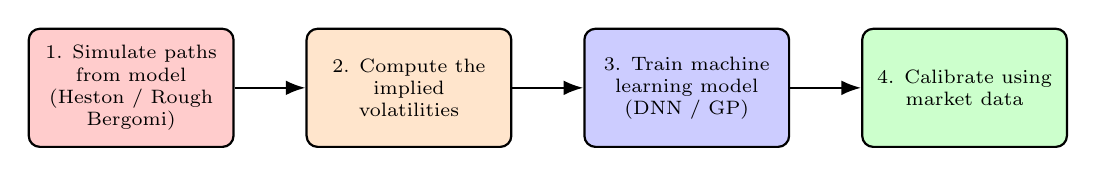
\begin{tikzpicture}[
    box/.style={rectangle, rounded corners, draw=black, thick,
                minimum width=2.6cm, minimum height=1.5cm,
                align=center, font=\scriptsize},
    arrow/.style={-{Latex[length=2.5mm]}, thick}
  ]
  \node[box, fill=red!20]    (b1) {1. Simulate paths\\from model\\(Heston / Rough\\Bergomi)};
  \node[box, fill=orange!20, right=0.9cm of b1] (b2) {2. Compute the\\implied\\volatilities};
  \node[box, fill=blue!20,   right=0.9cm of b2] (b3) {3. Train machine\\learning model\\(DNN / GP)};
  \node[box, fill=green!20,  right=0.9cm of b3] (b4) {4. Calibrate using\\market data};

  \draw[arrow] (b1) -- (b2);
  \draw[arrow] (b2) -- (b3);
  \draw[arrow] (b3) -- (b4);
\end{tikzpicture}
\end{center}

\begin{block}{The Four Steps, Explained}
\begin{enumerate}
  \item \textbf{Simulate paths:} for a chosen set of model parameters,
        simulate synthetic asset/variance paths from Heston or Rough
        Bergomi.
  \item \textbf{Compute implied volatilities:} from the synthetic data,
        compute the corresponding option price or implied volatility --
        the training \emph{label} for that parameter vector. Any
        numerical pricing method (e.g.\ Monte Carlo) can be used here.
  \item \textbf{Train ML model:} learn the mapping
        (parameters) $\mapsto$ (implied volatility surface) using a
        machine learning model, \emph{offline}, on the simulated data.
  \item \textbf{Calibrate to market data:} with the trained (near-instant)
        surrogate in hand, find the parameters that best reproduce
        \emph{today's} real market surface using a standard calibration
        (optimization) routine.
\end{enumerate}
\end{block}
\end{frame}

\subsection{4.3.2 Deep Neural Networks and Gaussian Processes}

\begin{frame}[allowframebreaks]{4.3.2 Deep Neural Networks as a Surrogate}

Neural networks are universal function approximators, and this chapter
uses a fully connected feed-forward deep network to learn the mapping
from model parameters to the (flattened) implied volatility surface.

\begin{block}{Feed-Forward Network (Eqs.\ 4.3--4.4)}
\[
  f_k(x) = b_k + \sum_j v_{jk}\,h_j(x)
\]
\[
  h_j(x) = \Psi\!\left(a_j + \sum_i w_{ij}\,x_i\right)
\]
where:
\begin{itemize}
  \item $x = (x_1,\ldots,x_i,\ldots)$ -- the input vector, here the
        stochastic volatility model's parameters (e.g.\
        $\{\kappa,\theta,\xi,\rho,v_0\}$ for Heston);
  \item $w_{ij}$ -- the weight connecting the $i$-th input to the $j$-th
        hidden unit;
  \item $a_j, b_k$ -- bias terms for hidden unit $j$ and output unit $k$;
  \item $\Psi$ -- the (non-linear) \textbf{activation function} that
        gives the network its ability to approximate non-linear
        pricing/implied-volatility maps;
  \item $h_j(x)$ -- the activation of the $j$-th hidden unit;
  \item $v_{jk}$ -- the weight from hidden unit $j$ to output unit $k$;
  \item $f_k(x)$ -- the $k$-th output, here the model-implied volatility
        at the $k$-th point of the (flattened) surface grid.
\end{itemize}
\end{block}

\framebreak

\textbf{Architecture used in this chapter:} three hidden layers, each
with 30 neurons, with an ELU activation function; a linear output layer
whose number of nodes equals the number of points on the volatility
surface (e.g.\ 30 for the FTSE/JSE ALSI grid, 88 for the EuroStoxx 50
grid -- see Sec.\ 4.4.1). This architecture mirrors the one proposed in
the deep calibration paper of Horv\'ath et al.\ (2021).

\begin{alertblock}{Strengths and Weaknesses of the DNN Surrogate}
\begin{itemize}
  \item \textbf{Strength:} once trained, evaluation is extremely fast --
        orders of magnitude faster than repeatedly running Monte Carlo,
        which is why DNN-based calibration is the current
        state-of-the-art speed benchmark.
  \item \textbf{Weakness:} no canonical way to choose the architecture;
        black-box, hard to interpret; and crucially, a plain DNN gives a
        single point-estimate prediction with \emph{no} uncertainty
        quantification.
\end{itemize}
\end{alertblock}

\end{frame}

\begin{frame}[allowframebreaks]{4.3.2 What Is a Gaussian Process?}

\begin{block}{Plain-Language Definition}
A neural network fits \emph{one} function to the data (one specific curve
of best fit). A \textbf{Gaussian process (GP)} instead puts a probability
distribution directly over \emph{functions}: rather than picking a single
best-fit curve, you get a whole \emph{distribution} of plausible curves
consistent with the data, together with an uncertainty band around them
that is naturally \emph{wide} wherever you have little or no data, and
\emph{narrow} near observed data points.
\end{block}

Formally, a Gaussian process is a set of random variables, any finite
subset of which is jointly (multivariate) Gaussian distributed. A GP is a
\textbf{prior over functions}. It is fully specified by two things:

\begin{itemize}
  \item a \textbf{mean function} $\mu(x')$ -- our best guess for $f(x')$
        before seeing any data (often taken to be zero or a constant);
  \item a \textbf{kernel (covariance) function} $k(x_i', x_j')$ -- encodes
        how similar/correlated we believe $f$ at two input points $x_i'$
        and $x_j'$ should be (e.g.\ nearby inputs $\Rightarrow$ similar
        function values, for a smooth kernel).
\end{itemize}

\framebreak

\textbf{Why does this matter for calibration?} Unlike a deep neural
network, once we've fit a GP surrogate for the pricing/implied-vol map, we
get \emph{uncertainty bands} on both the surrogate's predictions and (by
propagating through the calibration routine) on the fitted model
parameters themselves -- valuable information a point-estimate network
simply cannot provide.

\textbf{Cost:} training a GP requires inverting an $n\times n$ kernel
matrix built from all $n$ training points -- an $O(n^3)$ operation. This
is the key computational bottleneck that motivates the
\textbf{sparse} Gaussian process machinery introduced later in this
section.

\end{frame}

\begin{frame}[allowframebreaks]{4.3.2 GP Regression: Posterior Mean and Variance}

Given a training dataset $\{\mathbf{x}_i', \mathbf{x}_t\}_{t=1}^{t}$ with
$t$ \emph{noisy} observations $\mathbf{x}_t = f(\mathbf{x}_t') + \epsilon$,
$\epsilon \sim \mathcal{N}(0, \sigma_X^2)$, the GP prior on $f$ implies
$f(\mathbf{x}') \sim \mathcal{N}(\mu_{\mathbf{x}'}, \mathbf{K}_{x'} +
\sigma_X^2\mathbf{I})$.

\begin{alertblock}{Notation Note}
This chapter's own notation uses $\mathbf{X}$ for the (noisy) observed
\emph{outputs} and $\mathbf{x}'$ for the \emph{inputs} -- the reverse of
many textbooks' convention (which often use $X$ for inputs, $y$ for
outputs). We reproduce the book's equations exactly below, then re-derive
the same result with the more common $x$-inputs/$y$-outputs notation on
the following slide to avoid any confusion.
\end{alertblock}

\begin{block}{Posterior Mean and Variance (Eqs.\ 4.5--4.6)}
\[
  \mathbb{E}(f_*) = \mu_{\mathbf{x}_*'} +
    k_*\left(K_{x'} + \sigma_X^2\mathbf{I}\right)^{-1}
    \left(\mathbf{X} - \mu_{\mathbf{x}'}\right)
\]
\[
  \operatorname{var}(f_*) = k_{**} -
    k_*^{\top}\left(K_{x'} + \sigma_X^2\mathbf{I}\right)^{-1} k_*
\]
where $k_{**} = k(\mathbf{x}_*', \mathbf{x}_*')$ (prior variance at the
test point) and $k_* = k(\mathbf{x}', \mathbf{x}_*')$ (covariances
between all training inputs and the test input).
\end{block}

\begin{block}{Hyperparameter Fitting (Eq.\ 4.7)}
\[
  \log p(\mathbf{X}\mid\mathbf{X}') =
    \log \mathcal{N}\!\left(\mu_{x'}, \mathbf{K}_{x'x'} + \sigma_X^2\mathbf{I}\right)
\]
The kernel hyperparameters (e.g.\ lengthscale, signal variance) and the
noise level $\sigma_X$ are found by maximizing this
\textbf{log-marginal likelihood} -- i.e.\ by asking which hyperparameters
make the \emph{observed} data most probable under the GP model.
\end{block}

\end{frame}

\begin{frame}[allowframebreaks]{Step-by-Step: Deriving the GP Posterior (Standard Notation)}

Let's rebuild the same result with cleaner, more standard notation:
inputs $x_1,\ldots,x_n$, noisy targets $y_i = f(x_i) + \epsilon_i$ with
$\epsilon_i \sim \mathcal{N}(0,\sigma_n^2)$ i.i.d., and a test input
$x_*$. Assume (for simplicity) a zero mean function.

\textbf{Step 1 -- Joint distribution.} Under the GP prior, the training
targets $\mathbf{y}=(y_1,\ldots,y_n)^\top$ and the (noise-free) function
value $f_*$ at the test point are \emph{jointly Gaussian}:
\[
  \begin{bmatrix} \mathbf{y} \\ f_* \end{bmatrix}
  \sim \mathcal{N}\!\left(\mathbf{0},
  \begin{bmatrix} K + \sigma_n^2 I & \mathbf{k}_* \\
                  \mathbf{k}_*^\top & k_{**} \end{bmatrix}\right)
\]
where $K_{ij}=k(x_i,x_j)$, $(\mathbf{k}_*)_i = k(x_i,x_*)$, and
$k_{**}=k(x_*,x_*)$.

\framebreak

\textbf{Step 2 -- Condition on the observed data.} Using the standard
formula for conditioning a joint Gaussian on part of its variables gives
the predictive distribution $f_* \mid \mathbf{y}$:
\[
  \mathbb{E}[f_*\mid\mathbf{y}] = \mathbf{k}_*^\top (K+\sigma_n^2 I)^{-1}\mathbf{y}
\]
\[
  \operatorname{Var}[f_*\mid\mathbf{y}] = k_{**} -
   \mathbf{k}_*^\top (K+\sigma_n^2 I)^{-1}\mathbf{k}_*
\]

This is exactly the structure of the book's Eqs.\ (4.5)--(4.6): the
posterior mean is a weighted combination of the observed targets (weights
determined by how correlated each training input is with the test
input, and de-noised via $\sigma_n^2$), and the posterior variance is the
\emph{prior} variance $k_{**}$ \emph{shrunk} by an amount that grows with
how much relevant training data ($\mathbf{k}_*$) we have nearby.

\textbf{Key intuition:} far from any training data, $\mathbf{k}_*\approx
\mathbf{0}$ (nothing correlates with the test point), so the mean reverts
to the prior mean (zero here) and the variance reverts to the prior
variance $k_{**}$ -- i.e.\ maximal uncertainty. Near training data, the
opposite happens: high confidence, narrow uncertainty band.

\end{frame}

\begin{frame}[allowframebreaks]{Worked Numeric Example: GP Posterior by Hand}

Let's compute an exact (small, non-sparse) GP posterior with just
\textbf{3 training points}, using the \textbf{squared exponential kernel}
$k(x,x')=\sigma_f^2\exp\!\left(-\tfrac12 (x-x')^2/\ell^2\right)$ with
$\sigma_f=1$, lengthscale $\ell=1$, and noise $\sigma_n=0.1$.

\begin{block}{Data}
$x = (-1, 0, 1)$, $\quad y = (0.9,\ 0.0,\ -0.9)$ $\quad$ (roughly $y\approx -x$),
$\quad$ test point $x_*=0.5$.
\end{block}

\textbf{Step 1: build $K+\sigma_n^2 I$.} Using
$k(-1,0)=k(0,1)=e^{-0.5}\approx 0.6065$ and $k(-1,1)=e^{-2}\approx 0.1353$:
\[
  K + \sigma_n^2 I =
  \begin{pmatrix}
    1.0100 & 0.6065 & 0.1353 \\
    0.6065 & 1.0100 & 0.6065 \\
    0.1353 & 0.6065 & 1.0100
  \end{pmatrix}
\]
(the $1.01 = \sigma_f^2+\sigma_n^2 = 1 + 0.01$ on the diagonal).

\framebreak

\textbf{Step 2: build $\mathbf{k}_*$ and $k_{**}$.}
\[
  \mathbf{k}_* = \big(k(-1,0.5),\ k(0,0.5),\ k(1,0.5)\big)
              = (0.3247,\ 0.8825,\ 0.8825), \qquad k_{**}=1.0
\]

\textbf{Step 3: solve the linear system and combine.} Solving
$(K+\sigma_n^2 I)\,\boldsymbol{\alpha} = \mathbf{y}$ for $\boldsymbol{\alpha}$
and then computing $\mathbf{k}_*^\top\boldsymbol{\alpha}$ (equivalent to the
formulas above) gives:
\begin{block}{Result (verified numerically)}
\[
  \mathbb{E}[f_*\mid\mathbf{y}] \approx -0.5740,
  \qquad
  \operatorname{Var}[f_*\mid\mathbf{y}] \approx 0.0250,
  \qquad
  \text{std} \approx 0.1582
\]
\end{block}

\textbf{Sanity check:} the true underlying trend is $y\approx -x$, so at
$x_*=0.5$ we would guess $y\approx -0.5$; the GP posterior mean
$-0.574$ is close to this but pulled slightly by the noisy training
values and the kernel's smoothing, exactly as expected, with a modest
posterior uncertainty because $x_*=0.5$ sits between two training points.

\end{frame}

\begin{frame}[allowframebreaks]{4.3.2 Sparse Gaussian Processes: Why and How}

\begin{block}{The Problem}
Exact GP training/inference costs $O(n^3)$ in the number of training
points $n$ (from inverting the $n\times n$ kernel matrix). This chapter's
experiments simulate \textbf{40{,}000} training smiles per model
(Sec.\ 4.4.2) -- far too many for an exact GP to handle directly.
\end{block}

\begin{block}{Plain-Language Fix: Inducing Points}
A \textbf{sparse Gaussian process} makes GPs tractable on large datasets
by summarizing the data with a small number of well-chosen
\textbf{``pseudo-points''} (also called \textbf{inducing points}),
$m \ll n$. Instead of inverting an $n\times n$ matrix, the model only ever
needs to invert $m\times m$ matrices, dramatically lowering both the
computational and memory cost -- at the price of an
\emph{approximation}.
\end{block}

\begin{itemize}
  \item The number of inducing points controls the quality of the
        approximation: more inducing points $\Rightarrow$ better
        approximation of the true (full) GP, but higher cost -- the user
        gets to trade off memory/compute against accuracy.
  \item Because sparse GPs typically lack a closed-form solution, they
        are trained via \textbf{variational inference}: Bayesian
        inference reframed as an optimization problem, maximizing a
        lower bound on the log-marginal likelihood.
\end{itemize}

\framebreak

\textbf{Single-output vs.\ multi-output sparse GPs (as used in this
chapter):}
\begin{itemize}
  \item \textbf{Single-output sparse GP:} fit one independent sparse GP
        \emph{per point} on the volatility surface grid (e.g.\ 30
        separate small GPs for the ALSI grid).
  \item \textbf{Multi-output sparse GP:} fit \emph{one} sparse GP that
        jointly models the \emph{whole surface at once} as a
        vector-valued output, allowing the model to implicitly learn
        connectivity/correlation between different points on the
        surface. In this chapter, the inducing points and kernel are
        \emph{shared} across all outputs of the multi-output GP.
  \item Both variants here use the \textbf{squared exponential kernel}.
\end{itemize}

This chapter's numerical experiments (Sec.\ 4.4--4.5) compare both sparse
GP variants against the deep neural network surrogate of Sec.\ 4.3.2.

\end{frame}

\begin{frame}{Toy Running Example: Sparse GP Fit to a Synthetic Smile}
\begin{columns}
  \column{0.5\textwidth}
    \textbf{Our own illustrative simulation} (not from the book): 24 noisy
    synthetic (strike, implied-vol) points sampled around a toy smile,
    fit with a sparse GP using just \textbf{5 inducing points}
    (squared-exponential kernel, lengthscale $\approx 16$).
    \vspace{4pt}

    \textbf{Numeric summary} (posterior mean $\pm$ std):
    \begin{itemize}
      \small
      \item near data-rich centre ($K=100$): mean $\approx 0.184$,
            std $\approx 0.005$ -- \emph{narrow} band;
      \item near the edges ($K=70,130$, sparser data): mean $\approx
            0.28,\ 0.13$, std $\approx 0.04$ -- \emph{wider} band.
    \end{itemize}
    This is the hallmark GP behaviour: uncertainty shrinks near data
    (and near inducing points) and grows away from it.
  \column{0.5\textwidth}
    \centering
    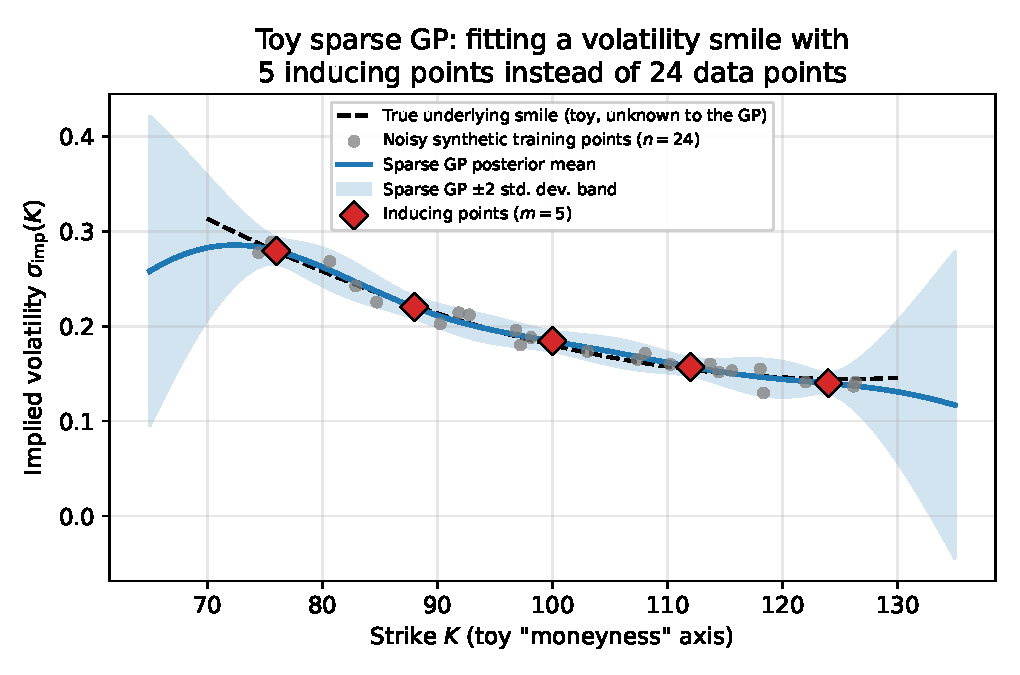
\includegraphics[width=\textwidth]{toy_sparse_gp}
\end{columns}
\end{frame}

\begin{frame}[fragile]{Python: A Sparse GP (DTC Approximation) From Scratch}
\begin{lstlisting}[style=python]
import numpy as np

def se_kernel(x1, x2, ell, sigma_f):
    """Squared exponential kernel k(x,x') = sigma_f^2 exp(-0.5(x-x')^2/ell^2)."""
    d2 = (x1.reshape(-1, 1) - x2.reshape(1, -1)) ** 2
    return sigma_f**2 * np.exp(-0.5 * d2 / ell**2)

def sparse_gp_predict(x_train, y_train, x_inducing, x_star,
                       ell, sigma_f, sigma_n):
    """Sparse GP regression via the Deterministic Training Conditional (DTC)
    approximation: only m x m matrices (m = number of inducing points) are
    ever inverted, instead of the full n x n kernel matrix."""
    Kmm = se_kernel(x_inducing, x_inducing, ell, sigma_f) + 1e-6 * np.eye(len(x_inducing))
    Knm = se_kernel(x_train, x_inducing, ell, sigma_f)
    Ksm = se_kernel(x_star, x_inducing, ell, sigma_f)

    Kmm_inv = np.linalg.inv(Kmm)
    Sigma = Kmm + (Knm.T @ Knm) / sigma_n**2       # only m x m to invert
    Sigma_inv = np.linalg.inv(Sigma)

    mean = (Ksm @ Sigma_inv @ (Knm.T @ y_train)) / sigma_n**2
    var = (sigma_f**2
           - np.einsum('ij,jk,ik->i', Ksm, Kmm_inv, Ksm)
           + np.einsum('ij,jk,ik->i', Ksm, Sigma_inv, Ksm))
    return mean, np.sqrt(np.clip(var, 1e-10, None))

# 5 inducing points summarising 24 noisy training observations (toy example)
x_inducing = np.array([76., 88., 100., 112., 124.])
mean, std = sparse_gp_predict(x_train, y_train, x_inducing, x_star,
                               ell=16.0, sigma_f=0.20, sigma_n=0.012)
\end{lstlisting}
\end{frame}

% ==============================================================================
\section{4.4 Numerical Experiments}
% ==============================================================================

\subsection{4.4.1 Data Description}

\begin{frame}[allowframebreaks]{4.4.1 Data Description: Two Equity Markets}

Real option market data from \textbf{100 consecutive trading days in
2019} is used for both markets, giving a like-for-like comparison of a
developing and a developed market.

\begin{block}{FTSE/JSE ALSI Option Data (South Africa -- Developing Market)}
Implied volatilities on a discrete 2-D grid of moneyness $M$ and time to
maturity $T$:
\[
  M := \{80\%, 90\%, 100\%, 110\%, 120\%\}, \qquad
  T := \{1M, 2M, 3M, 6M, 9M, 1Y\}
\]
giving $5 \times 6 = \mathbf{30}$ points on each implied volatility
surface. Calibrated using the \textbf{Heston} model.
\end{block}

\begin{block}{EuroStoxx 50 Option Data (Europe -- Developed Market)}
\[
  M := \{50\%,60\%,\ldots,150\%\}\ (11\text{ values, step }10\%), \qquad
  T := \{0.1Y, 0.3Y, 0.6Y, 0.9Y, 1.2Y, 1.5Y, 1.8Y, 2.0Y\}\ (8\text{ values})
\]
giving $11 \times 8 = \mathbf{88}$ points on each implied volatility
surface. Calibrated using the \textbf{Rough Bergomi} model.
\end{block}

\framebreak

\textbf{Why pair Heston with ALSI and Rough Bergomi with EuroStoxx?} This
mirrors the chapter's aim of demonstrating the Bayesian (sparse GP)
calibration framework across \emph{both} a classical, tractable model on
a developing market, and a modern rough-volatility model on a developed
market -- rather than an exhaustive cross-product of every
model/market combination.

Note also the very different \emph{grid sizes}: 30 points for ALSI vs.\
88 for EuroStoxx. This directly affects the machine learning surrogates'
output dimensionality (Sec.\ 4.3.2, 4.4.2) -- e.g.\ the neural network's
number of output nodes must match the grid size for each market.

\end{frame}

\subsection{4.4.2 Experiment Description}

\begin{frame}[allowframebreaks]{4.4.2 Experiment Description: Training and Calibration Setup}

\begin{block}{Offline Training Data (Simulated)}
For each stochastic volatility model, \textbf{40{,}000 training
examples} were simulated: 40{,}000 Heston smiles, and (separately)
40{,}000 Rough Bergomi smiles. Each example pairs a parameter vector with
its resulting implied volatility surface (computed numerically, e.g.\ via
Monte Carlo where needed).
\end{block}

\begin{block}{Machine Learning Models Compared}
\begin{itemize}
  \item \textbf{Deep neural network (DNN):} 3 hidden layers of 30 neurons
        each, \textbf{ELU} activation, linear output layer; number of
        output nodes = surface size (30 for ALSI, 88 for EuroStoxx).
  \item \textbf{Single-output sparse GP:} one sparse GP per surface
        point, squared exponential kernel, \textbf{100 inducing points}
        each.
  \item \textbf{Multi-output sparse GP:} one joint sparse GP over the
        whole surface, squared exponential kernel,
        \textbf{1{,}000 inducing points}.
\end{itemize}
\end{block}

\framebreak

\begin{block}{Online Calibration and Evaluation}
All three trained models are then calibrated \emph{online} to the real
FTSE/JSE ALSI and EuroStoxx 50 market data (100 trading days each), using
a standard calibration routine against the (now near-instant) surrogate.
Performance is assessed using the \textbf{root mean square error (RMSE)}
across the \emph{entire} volatility surface, together with the
computational resources required by each method.
\end{block}

All results in the book were produced in Python on a 64-bit machine.

\end{frame}

\begin{frame}[fragile]{Python: Training-Data Simulation \& Surrogate Pipeline}
\begin{lstlisting}[style=python]
import numpy as np

def build_training_set(n_examples, simulate_fn, price_to_impliedvol_fn,
                        strikes, maturities, seed=0):
    """Steps 1-2 of the calibration framework: simulate model paths for
    randomly sampled parameter vectors, then convert to an implied
    volatility surface (the training label)."""
    rng = np.random.default_rng(seed)
    X_params, Y_surfaces = [], []
    for _ in range(n_examples):
        theta = sample_parameter_vector(rng)          # e.g. Heston/RoughBergomi params
        paths = simulate_fn(theta, strikes, maturities)
        iv_surface = price_to_impliedvol_fn(paths, strikes, maturities)
        X_params.append(theta)
        Y_surfaces.append(iv_surface.flatten())
    return np.array(X_params), np.array(Y_surfaces)

# Step 3: train a surrogate offline (DNN shown; GP analogous, see prior slide)
X_train, Y_train = build_training_set(40_000, simulate_heston,
                                       price_to_impliedvol, strikes, maturities)
surrogate = train_dnn(X_train, Y_train, hidden=(30, 30, 30), activation='elu')

# Step 4: calibrate to real market data using the fast surrogate
from scipy.optimize import minimize
market_surface = load_market_iv_surface('ALSI')   # 30-point grid
loss = lambda theta: np.sqrt(np.mean((surrogate.predict(theta) - market_surface) ** 2))
result = minimize(loss, x0=initial_guess, method='Nelder-Mead')
print("Calibrated parameters:", result.x, " RMSE:", result.fun)
\end{lstlisting}
\end{frame}

% ==============================================================================
\section{4.5 Results and Discussion}
% ==============================================================================

\begin{frame}[allowframebreaks]{4.5 Speed and Parameter Stability}

\begin{block}{Computational Speed}
As expected, the \textbf{deep neural network was the fastest} method. The
\textbf{single-output sparse GP was the slowest}, at around
\textbf{6 times slower} than the DNN. This highlights the main practical
drawback of the GP approach: even with sparsity, GP training/evaluation
remains more expensive than a neural network, motivating future work on
distributed/scalable GP methods.
\end{block}

\begin{block}{Parameter Stability Over Time (Heston on FTSE/JSE ALSI)}
All three methods (multi-output sparse GP, DNN, single-output sparse GP)
produce \emph{similar} Heston parameter estimates across the 100 trading
days for most parameters. The \textbf{deep neural network showed the
most instability} in its parameter estimates through time, particularly
for $\nu$ and $\theta$ -- i.e.\ the DNN's calibrated parameters jumped
around more from day to day than the GP-based methods' did.
\end{block}

\framebreak

\textbf{Why might the GP-based methods be more stable?} Because GPs are
Bayesian, their predictions (and hence their implied calibration loss
surface) are naturally smoothed/regularized relative to a plain
point-estimate neural network -- one of the practical benefits motivating
this chapter's Bayesian framework, beyond simply reporting uncertainty
bands.

\end{frame}

\begin{frame}[allowframebreaks]{4.5 Fit Quality: Best- and Worst-Calibration Days}

\textbf{On the days with the largest calibration error} (for each
market): in general all three methods produce very similar fits to the
data, \emph{except} for the multi-output sparse GP, whose fit visibly
deviates from the other two as maturity increases. The two GP approaches
show similar confidence bands on the ALSI dataset, though the
single-output GP produces noticeably \emph{narrower} (lower)
one-standard-deviation bands than the multi-output GP.

For the \textbf{smallest maturity} on the EuroStoxx 50 data, \emph{all
three} methods fail to fully capture the skew around the at-the-money
point on the worst day -- this particular skew was unusually steep
compared to the market's typical skew over the study period.

\framebreak

Across both datasets, a consistent pattern emerges in the
\textbf{confidence bands}: the \emph{lowest} maturity has the
\emph{narrowest} confidence bands overall, with bands widening as
maturity increases; and within a given maturity, bands are narrowest
around the at-the-money moneyness level, widening as one moves away from
at-the-money.

\textbf{On the days with the smallest calibration error}, all three
methods fit the data noticeably better -- in particular, all three fully
capture the EuroStoxx 50 skew at the smallest maturity on these
``easy'' days (in contrast to the worst-day case above). The
multi-output GP's fit still deviates from the other two as maturity
increases, and the same pattern of narrower bands at low maturity /
wider bands at high maturity persists.

\end{frame}

\begin{frame}[allowframebreaks]{4.5 RMSE Through Time and Overall Ranking}

\begin{block}{RMSE Across the Whole Surface, Over Time}
Tracking the root mean square error across the entire volatility surface
through all 100 trading days shows that the calibration error is fairly
stable for all three methods, though there are periods with noticeably
larger errors -- possibly indicating that a larger training set, or a
different/better-specified stochastic volatility model, would be needed
on those particular days.
\end{block}

\begin{block}{Which Method Performs Worst Overall?}
On \emph{both} datasets, the \textbf{multi-output sparse GP is the
poorest performer}, with a consistently higher RMSE than the other two
methods through time. This is explained by its comparatively poor fit at
\textbf{large maturities} on the volatility surface, as noted in the
smile-by-smile comparisons above. On the FTSE/JSE ALSI data specifically,
the DNN and single-output GP track each other closely; on EuroStoxx 50,
the single-output GP performs similarly to the DNN, with the multi-output
GP trailing well behind both.
\end{block}

\framebreak

\begin{alertblock}{The Headline Result}
The (Bayesian, sparse GP) probabilistic approach achieves \textbf{similar
predictive performance to the deep neural network} -- the current
state-of-the-art -- while additionally providing calibrated
\textbf{uncertainty estimates} on both the fitted volatility surface and
(by extension) the calibrated model parameters. This is valuable to
practitioners who need to understand not just their best single estimate
of the smile shape, but how confident they should be in it across
different maturities.
\end{alertblock}

\end{frame}

\begin{frame}{4.5 Toy Illustration vs.\ the Book's Real-Market Results}
  \begin{block}{Keep These Two Firmly Separate}
    \begin{itemize}
      \item \textbf{Our toy example} (earlier in Sec.\ 4.3.2): a
            synthetic, hand-constructed smile with 24 noisy points and
            \textbf{5} inducing points -- built purely to give visual and
            numerical intuition for how a sparse GP posterior behaves.
      \item \textbf{The book's actual experiment} (this section): real
            FTSE/JSE ALSI and EuroStoxx 50 market data over
            \textbf{100 trading days}, with \textbf{40{,}000} simulated
            training smiles per stochastic volatility model, and
            \textbf{100} (single-output) or \textbf{1{,}000}
            (multi-output) inducing points.
    \end{itemize}
  \end{block}
  The scales are wildly different, but the \emph{mechanism} is identical:
  a handful of well-placed inducing points summarizing a much larger
  dataset, producing a posterior mean and an uncertainty band that
  widens where data (or inducing points) are sparse -- exactly what our
  toy figure shows on a small scale, and what the book's real-market
  results show at production scale.
\end{frame}

% ==============================================================================
\section{4.6 Conclusion}
% ==============================================================================

\begin{frame}[allowframebreaks]{4.6 Conclusion}

This chapter used \textbf{sparse Gaussian processes} to calibrate the
Heston and Rough Bergomi stochastic volatility models to real option
volatility data across a developing market (FTSE/JSE ALSI) and a
developed market (EuroStoxx 50). Both single-output (per-surface-point)
and multi-output (whole-surface-at-once) sparse GPs were considered, and
benchmarked against the current state-of-the-art deep neural network
approach.

\begin{block}{Key Findings}
\begin{itemize}
  \item The (Bayesian) probabilistic approach produces results
        \textbf{similar} to the deep neural network, with the added
        advantage of \textbf{capturing uncertainty} in the calibration.
  \item On the \textbf{FTSE/JSE ALSI} data, the single- and multi-output
        GPs produce similar results, with narrow confidence bands at
        lower moneyness/maturity and wider bands as moneyness and
        maturity increase.
  \item On the \textbf{EuroStoxx 50} data, the multi-output GP is the
        poorest performer, with visibly wide confidence bands reflecting
        this; the single-output GP produces results similar to the
        neural network, with narrower confidence bands than the
        multi-output GP.
\end{itemize}
\end{block}

\framebreak

\begin{alertblock}{Limitations and Future Work}
\begin{itemize}
  \item \textbf{Shared inducing points/kernel:} the multi-output GP's
        weaker EuroStoxx 50 performance may be improved by \emph{not}
        sharing inducing points and kernels across the surface's output
        dimensions.
  \item \textbf{No explicit no-arbitrage constraints:} like the neural
        network literature this chapter compares against, the
        approximated pricing function is not guaranteed to be
        arbitrage-free. Incorporating no-arbitrage conditions explicitly
        is left to future work.
  \item \textbf{Computational cost:} the main drawback of the GP
        approach versus neural networks remains its higher computational
        complexity (recall: single-output GP $\approx 6\times$ slower
        than the DNN). Future work will explore
        \textbf{distributed/scalable GP} approaches (e.g.\
        product-of-experts methods) to address this.
\end{itemize}
\end{alertblock}

\end{frame}

\begin{frame}{4.6 Looking Ahead}
  \begin{block}{Where This Chapter Sits in the Bigger Picture}
    Model calibration here relied on a \emph{formal} stochastic
    volatility model (Heston or Rough Bergomi) plus a machine learning
    surrogate to speed up fitting it to data -- and, as just discussed,
    this approach does not automatically guarantee arbitrage-free prices.
  \end{block}
  \begin{alertblock}{Next Chapter Preview}
    The next chapter takes a different route: a \textbf{normalizing
    flows}-based approach to pricing options in an emerging market. By
    learning the \textbf{risk-neutral density} directly, this approach
    does not need to impose no-arbitrage conditions as an extra
    constraint on a loss function -- the learned density already
    captures them by construction.
  \end{alertblock}
\end{frame}

\end{document}
